% EGE 2027, task 11. Source IDs and URLs are kept in comments.
% Editable task bank. Append new BankTask blocks at the end of the document.
\documentclass[12pt,a4paper]{article}
\usepackage{physics-textbook}
\usepackage{graphicx,needspace}
\newif\ifShowSolutions
\ifdefined\TutorEdition
  \ShowSolutionstrue
\else
  \ShowSolutionsfalse
\fi
\newcounter{banktask}
\newcommand{\BankTask}[3]{%
  \refstepcounter{banktask}%
  \Needspace{35mm}\par\medskip\noindent\begin{minipage}{\linewidth}%
  \noindent\textbf{\thebanktask.}\quad #2\par
  \ifShowSolutions
    #3\par
    \ifdefined\TutorEdition
      \ifcsname TutorSource#1\endcsname
        \smallskip{\small\csname TutorSource#1\endcsname\par}%
      \fi
    \fi
  \fi
  \end{minipage}\par\medskip
}
\begin{document}
Справочные величины (если в условии не оговорено иное):\par
$k_{\text{К}}=9\cdot10^9\,\text{Н}\cdot\text{м}^2/\text{Кл}^2$



% Source 3BB12E: https://ege.fipi.ru/bank/questions.php?search=1&proj=BA1F39653304A5B041B656915DC36B38&qid=3BB12E
\BankTask{3BB12E}{
Одинаковые отрицательные точечные заряды, модуль которых $|q|=2\cdot10^{-8}\,\text{Кл}$, расположены в вакууме на расстоянии $3\,\text{м}$ друг от друга. Определите модуль сил взаимодействия этих зарядов друг с другом.

Ответ выразите в $\text{мкН}$. (в $\text{мкН}$).
}{
\smallskip\noindent\textbf{Решение от GPT}\par
По закону Кулона при $k_{\text{К}}=9\cdot10^9\,\text{Н}\cdot\text{м}^2/\text{Кл}^2$:
\[
F=k_{\text{К}}\frac{|q|^2}{r^2}=9\cdot10^9\frac{(2\cdot10^{-8})^2}{3^2}=4\cdot10^{-7}\,\text{Н}=0{,}4\,\text{мкН}.
\]
Ответ: $0{,}4\,\text{мкН}$.
}

% Source D48CE0: https://ege.fipi.ru/bank/questions.php?search=1&proj=BA1F39653304A5B041B656915DC36B38&qid=D48CE0
\BankTask{D48CE0}{
Два неподвижных заряженных шарика, находящихся в вакууме на расстоянии $0{,}3\,\text{м}$ друг от друга, притягиваются друг к другу с силой $8\cdot10^{-9}\,\text{Н}$. Чему равен модуль заряда второго шарика, если заряд первого составляет $2\cdot10^{-10}\,\text{Кл}$? Ответ выразите в нанокулонах ($\text{нКл}$). (в $\text{нКл}$).
}{
\smallskip\noindent\textbf{Решение от GPT}\par
По закону Кулона при $k_{\text{К}}=9\cdot10^9\,\text{Н}\cdot\text{м}^2/\text{Кл}^2$:
\[
|q_2|=\frac{Fr^2}{k_{\text{К}}|q_1|}=\frac{8\cdot10^{-9}\cdot(0{,}3)^2}{9\cdot10^9\cdot2\cdot10^{-10}}=4\cdot10^{-10}\,\text{Кл}=0{,}4\,\text{нКл}.
\]
Ответ: $0{,}4\,\text{нКл}$.
}

% Source 8FC4FE: https://ege.fipi.ru/bank/questions.php?search=1&proj=BA1F39653304A5B041B656915DC36B38&qid=8FC4FE
\BankTask{8FC4FE}{
Два неподвижных точечных заряда действуют друг на друга с силами, модуль которых равен $F$. Во сколько раз увеличится модуль этих сил, если оба заряда увеличить в $3$ раза, а расстояние между ними увеличить в $2$ раза?
}{
\smallskip\noindent\textbf{Решение от GPT}\par
По закону Кулона $F\propto |q_1q_2|/r^2$, поэтому
\[
\frac{F'}{F}=\frac{3\cdot3}{2^2}=\frac94=2{,}25.
\]
Ответ: в $2{,}25$ раза.
}

% Source 11272F: https://ege.fipi.ru/bank/questions.php?search=1&proj=BA1F39653304A5B041B656915DC36B38&qid=11272F
\BankTask{11272F}{
Во сколько раз уменьшится модуль сил взаимодействия двух небольших металлических шариков одинакового диаметра, имеющих заряды \(q_1=+7\,\text{нКл}\) и \(q_2=-3\,\text{нКл}\), если шарики привести в соприкосновение и раздвинуть на прежнее расстояние?
}{
\smallskip\noindent\textbf{Решение от GPT}\par
После соприкосновения заряды одинаковых шариков равны: \(q'=(q_1+q_2)/2=2\,\text{нКл}\). По закону Кулона при прежнем расстоянии
\[
\frac{F}{F'}=\frac{|q_1q_2|}{(q')^2}=\frac{7\cdot3}{2^2}=5{,}25.
\]
Ответ: уменьшится в \(5{,}25\) раза.
}

% Source 2583B9: https://ege.fipi.ru/bank/questions.php?search=1&proj=BA1F39653304A5B041B656915DC36B38&qid=2583B9
\BankTask{2583B9}{
\begin{center}
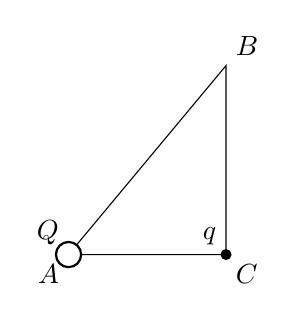
\begin{tikzpicture}[>=stealth,scale=1]
\coordinate (A) at (0,0);
\coordinate (C) at (2,0);
\coordinate (B) at (2,2.4);
\draw (A)--(B)--(C)--cycle;
\fill[white] (A) circle (0.16);
\draw[thick] (A) circle (0.16);
\fill (C) circle (0.07);
\node[below left] at (A) {$A$};
\node[above left] at (A) {$Q$};
\node[below right] at (C) {$C$};
\node[above left] at (C) {$q$};
\node[above right] at (B) {$B$};
\end{tikzpicture}
\end{center}
В треугольнике \(ABC\) угол \(C\) прямой, \(BC=0{,}8\,\text{м}\). В вершине \(A\) находится точечный заряд \(Q\). Он действует с силой \(2{,}5\cdot10^{-8}\,\text{Н}\) на точечный заряд \(q\), помещённый в вершину \(C\). Если заряд \(q\) перенести в вершину \(B\), то заряды будут взаимодействовать с силой \(9{,}0\cdot10^{-9}\,\text{Н}\). Найдите \(AC\). (в $\text{м}$).
}{
\smallskip\noindent\textbf{Решение от GPT}\par
По закону Кулона \(F_C/F_B=AB^2/AC^2=25/9\). По теореме Пифагора \(AB^2=AC^2+BC^2\), поэтому
\[
\frac{25}{9}=1+\frac{0{,}8^2}{AC^2},\qquad
AC=\sqrt{\frac{0{,}64\cdot9}{16}}=0{,}6\,\text{м}.
\]
Ответ: \(0{,}6\,\text{м}\).
}

% Source D1ECFE: https://ege.fipi.ru/bank/questions.php?search=1&proj=BA1F39653304A5B041B656915DC36B38&qid=D1ECFE
\BankTask{D1ECFE}{
Сила тока, текущего по проводнику, равна \(6\ \text{А}\). Какой заряд пройдёт по проводнику за \(30\ \text{с}\) (в $\text{Кл}$)?
}{
\smallskip\noindent\textbf{Решение от GPT}\par
\(q=It=6\cdot30=180\ \text{Кл}\).

Ответ: \(180\ \text{Кл}\).
}

% Source 30BB4c: https://ege.fipi.ru/bank/questions.php?search=1&proj=BA1F39653304A5B041B656915DC36B38&qid=30BB4c
\BankTask{30BB4c}{
По проводнику течёт постоянный электрический ток. Величина заряда, прошедшего через поперечное сечение проводника, возрастает с течением времени согласно графику (см. рисунок). Определите силу тока в проводнике.

\begin{center}
\begin{tikzpicture}[x=0.8cm,y=4cm,>=stealth]
\draw[->] (0,0)--(5.25,0) node[below] {\(t,\text{с}\)};
\draw[->] (0,0)--(0,1.02) node[left] {\(q,\text{Кл}\)};
\foreach \x in {1,2,3,4}{
  \draw[thin] (\x,0.47)--(\x,0.88);
  \draw (\x,0)--(\x,0.055);
  \node[below] at (\x,0) {\(\x\)};
}
\foreach \y/\lab in {0.2/{0{,}2},0.4/{0{,}4},0.6/{0{,}6},0.8/{0{,}8}}{
  \draw[thin] (0,\y)--(2,\y);
  \draw[thin] (4.15,\y)--(4.6,\y);
  \node[left] at (0,\y) {\(\lab\)};
}
\node[below left] at (0,0) {\(0\)};
\draw[thick] (0,0)--(3,0.6);
\end{tikzpicture}
\end{center} (в $\text{А}$).
}{
\smallskip\noindent\textbf{Решение от GPT}\par
Сила тока равна наклону графика: \(I=\dfrac{\Delta q}{\Delta t}=\dfrac{0{,}6}{3}=0{,}2\ \text{А}\).

Ответ: \(0{,}2\ \text{А}\).
}

% Source 8EB8E6: https://ege.fipi.ru/bank/questions.php?search=1&proj=BA1F39653304A5B041B656915DC36B38&qid=8EB8E6
\BankTask{8EB8E6}{
\begin{center}
\begin{tikzpicture}[x=0.23cm,y=0.08cm,>=stealth]
\draw[thin] (0,10)--(20,10);
\draw[thin] (0,20)--(20,20);
\draw[thin] (0,30)--(20,30);
\foreach \x in {5,10,15,20}{\draw[thin] (\x,0)--(\x,30);}
\draw[->] (0,0)--(24,0) node[below] {\(t,\text{с}\)};
\draw[->] (0,0)--(0,39) node[left] {\(I,\text{мА}\)};
\foreach \x in {5,10,15,20}{\node[below] at (\x,0) {\(\x\)};}
\foreach \y in {10,20,30}{\node[left] at (0,\y) {\(\y\)};}
\node[below left] at (0,0) {\(0\)};
\draw[thick] (0,0)--(5,30)--(10,20)--(15,20)--(20,0);
\end{tikzpicture}
\end{center}

На рисунке показана зависимость силы тока \(I\) в проводнике от времени \(t\). Определите заряд, прошедший по проводнику за интервал времени от \(5\) до \(15\ \text{с}\). (в $\text{мКл}$).
}{
\smallskip\noindent\textbf{Решение от GPT}\par
Заряд равен площади под графиком тока за указанный интервал:
\[
q=\frac{30+20}{2}\cdot(10-5)+20\cdot(15-10)=225\ \text{мКл},
\]
так как \(1\ \text{мА}\cdot\text{с}=1\ \text{мКл}\).

Ответ: \(225\ \text{мКл}\).
}

% Source 648474: https://ege.fipi.ru/bank/questions.php?search=1&proj=BA1F39653304A5B041B656915DC36B38&qid=648474
\BankTask{648474}{
На рисунке показан график зависимости силы тока в проводнике от напряжения между его концами. Чему равно сопротивление проводника?
\begin{center}
\begin{tikzpicture}[x=0.48cm,y=0.48cm,>=stealth]
\draw[->] (0,0)--(12,0) node[right] {$U,\,\text{В}$};
\draw[->] (0,0)--(0,7.8) node[left] {$I,\,\text{А}$};
\foreach \x in {2,4,6,8,10} {
\foreach \a/\b in {0/0.55,1.85/3.15,4.5/5.8,5.98/6}\draw (\x,\a)--(\x,\b);
\draw (\x,0.12)--(\x,-0.12) node[below] {$\x$};
}
\foreach \y in {2,4,6} {
\foreach \a/\b in {0.22/1.48,2.84/4.10,5.46/6.72,8.09/9.35,9.9/10}\draw (\a,\y)--(\b,\y);
\draw (0.12,\y)--(-0.12,\y) node[left] {$\y$};
}
\node[below left] at (0,0) {$0$};
\draw[very thick] (0,0)--(10,3.3333);
\end{tikzpicture}
\end{center} (в $\text{Ом}$).
}{
\smallskip\noindent\textbf{Решение от GPT}\par
По графику при $U=6\,\text{В}$ сила тока $I=2\,\text{А}$. По закону Ома
\[
R=\frac{U}{I}=\frac{6}{2}=3\,\text{Ом}.
\]
Ответ: $3\,\text{Ом}$.
}

% Source De83D5: https://ege.fipi.ru/bank/questions.php?search=1&proj=BA1F39653304A5B041B656915DC36B38&qid=De83D5
\BankTask{De83D5}{
На рисунке показан график зависимости силы тока в лампе накаливания от напряжения на её клеммах. Определите мощность тока в лампе при силе тока, равной $1{,}5\,\text{А}$.
\begin{center}
\begin{tikzpicture}[x=0.15cm,y=1.5cm,>=stealth]
\draw[thin] (0,0) grid[xstep=5,ystep=0.5] (35,2.5);
\draw (0,0)--(35,0) node[right] {$U,\,\text{В}$};
\draw[->] (0,0)--(0,2.9) node[left] {$I,\,\text{А}$};
\node[below left] at (0,0) {$0$};
\foreach \x in {10,20,30} \node[below] at (\x,0) {$\x$};
\foreach \y in {1,2} \node[left] at (0,\y) {$\y$};
\draw[very thick] (0,0) .. controls (3,0.35) and (6.5,0.68) .. (10,0.94) .. controls (13.5,1.18) and (17,1.38) .. (20,1.5) .. controls (25,1.7) and (30,1.9) .. (35,2);
\end{tikzpicture}
\end{center} (в $\text{Вт}$).
}{
\smallskip\noindent\textbf{Решение от GPT}\par
По графику при $I=1{,}5\,\text{А}$ напряжение $U=20\,\text{В}$. Мощность тока:
\[
P=UI=20\cdot1{,}5=30\,\text{Вт}.
\]
Ответ: $30\,\text{Вт}$.
}

% Source 0990BD: https://ege.fipi.ru/bank/questions.php?search=1&proj=BA1F39653304A5B041B656915DC36B38&qid=0990BD
\BankTask{0990BD}{
При прохождении по проводнику постоянный электрический ток силой $3\,\text{А}$ в течение $60\,\text{с}$ совершает работу, равную $270\,\text{кДж}$. Чему равно сопротивление проводника (в $\text{Ом}$)?
}{
\smallskip\noindent\textbf{Решение от GPT}\par
Работа постоянного тока $A=I^2Rt$. Следовательно,
\[
R=\frac{A}{I^2t}=\frac{270\cdot10^3}{3^2\cdot60}=500\,\text{Ом}.
\]
Ответ: $500\,\text{Ом}$.
}

% Source 0AEE10: https://ege.fipi.ru/bank/questions.php?search=1&proj=BA1F39653304A5B041B656915DC36B38&qid=0AEE10
\BankTask{0AEE10}{
На колбе лампы накаливания указано: «\(165\ \text{Вт},\ 220\ \text{В}\)». Найдите силу тока в спирали при включении лампы в сеть с таким напряжением. (в $\text{А}$).
}{
\smallskip\noindent\textbf{Решение от GPT}\par
Из \(P=UI\) получаем
\[
I=\frac{P}{U}=\frac{165}{220}=0{,}75\ \text{А}.
\]
Ответ: \(0{,}75\ \text{А}\).
}

% Source D474CD: https://ege.fipi.ru/bank/questions.php?search=1&proj=BA1F39653304A5B041B656915DC36B38&qid=D474CD
\BankTask{D474CD}{
На плавком предохранителе указано: «\(30\ \text{А}\)». Какова максимальная суммарная мощность электрических приборов, которые можно одновременно включить в сеть с напряжением \(36\ \text{В}\), чтобы предохранитель не расплавился (в $\text{Вт}$)?
}{
\smallskip\noindent\textbf{Решение от GPT}\par
Суммарный ток не должен превышать \(I_{\max}=30\ \text{А}\). Поэтому
\[
P_{\max}=UI_{\max}=36\cdot30=1080\ \text{Вт}.
\]
Ответ: \(1080\ \text{Вт}\).
}

% Source F934C0: https://ege.fipi.ru/bank/questions.php?search=1&proj=BA1F39653304A5B041B656915DC36B38&qid=F934C0
\BankTask{F934C0}{
На участке цепи, изображённом на рисунке, сопротивление каждого из четырёх резисторов равно $6\,\text{Ом}$. Каково общее сопротивление цепи между клеммами $\text{А}$ и $\text{В}$?
\begin{center}
\begin{tikzpicture}[x=1cm,y=1cm,>=stealth,line width=0.8pt]
\draw (0,0) circle (0.06) node[left=4pt] {$\text{А}$};
\draw (0.06,0)--(0.8,0);
\draw (0.8,0)--(0.8,0.35)--(1.05,0.35);
\draw (1.05,0.18) rectangle (1.85,0.52);
\draw (1.85,0.35)--(2.1,0.35)--(2.1,0);
\draw (0.8,0)--(0.8,-0.35)--(1.05,-0.35);
\draw (1.05,-0.52) rectangle (1.85,-0.18);
\draw (1.85,-0.35)--(2.1,-0.35)--(2.1,0);
\fill (0.8,0) circle (0.055);
\fill (2.1,0) circle (0.055);
\draw (2.1,0)--(2.8,0);
\draw (2.8,-0.17) rectangle (3.6,0.17);
\draw (3.6,0)--(4.3,0);
\draw (4.3,-0.17) rectangle (5.1,0.17);
\draw (5.1,0)--(5.84,0);
\draw (5.9,0) circle (0.06) node[right=4pt] {$\text{В}$};
\end{tikzpicture}
\end{center} (в $\text{Ом}$).
}{
\smallskip\noindent\textbf{Решение от GPT}\par
Два левых резистора соединены параллельно, остальные — последовательно с ними:
\[
R_{\text{общ}}=\frac{6\cdot6}{6+6}+6+6=15\ \text{Ом}.
\]
Ответ: \(15\,\text{Ом}\).
}

% Source 849501: https://ege.fipi.ru/bank/questions.php?search=1&proj=BA1F39653304A5B041B656915DC36B38&qid=849501
\BankTask{849501}{
\begin{center}
\begin{tikzpicture}[x=1cm,y=1cm,>=stealth,line width=0.8pt]
\draw (0,1.6) circle (0.06) node[left=4pt] {$\text{А}$};
\draw (0.06,1.6)--(0.5,1.6);
\draw (0.5,1.43) rectangle (1.3,1.77);
\node[above] at (0.9,1.77) {\(R\)};
\draw (1.3,1.6)--(1.7,1.6)--(3.3,1.6)--(3.3,1.3);
\draw (1.7,1.6)--(1.7,1.3);
\draw (1.53,0.3) rectangle (1.87,1.3);
\node[left] at (1.53,0.8) {\(R\)};
\draw (1.7,0.3)--(1.7,0);
\draw (3.13,0.3) rectangle (3.47,1.3);
\node[right] at (3.47,0.8) {\(R\)};
\draw (3.3,0.3)--(3.3,0)--(0.06,0);
\draw (0,0) circle (0.06) node[left=4pt] {$\text{В}$};
\draw (1.7,1.6)--(2.35,0.95);
\draw (2.35,0.95)--(2.85,0.9);
\draw (2.65,0.65)--(3.3,0);
\node at (2.55,1.17) {$\text{К}$};
\fill (1.7,1.6) circle (0.045);
\fill (1.7,0) circle (0.045);
\fill (3.3,0) circle (0.045);
\end{tikzpicture}
\end{center}
На сколько уменьшится сопротивление участка цепи $\text{АВ}$, изображённого на рисунке, если ключ $\text{К}$ замкнуть? Сопротивление каждого резистора $R=2\,\text{Ом}$ (в $\text{Ом}$).
}{
\smallskip\noindent\textbf{Решение от GPT}\par
При разомкнутом ключе два вертикальных резистора соединены параллельно:
\[
R_{\text{разомк}}=R+\frac{R}{2}=3\ \text{Ом}.
\]
Замкнутый ключ закорачивает оба вертикальных резистора, поэтому \(R_{\text{замк}}=R=2\ \text{Ом}\). Уменьшение сопротивления:
\[
\Delta R=3-2=1\ \text{Ом}.
\]
Ответ: \(1\,\text{Ом}\).
}

% Source A5D05E: https://ege.fipi.ru/bank/questions.php?search=1&proj=BA1F39653304A5B041B656915DC36B38&qid=A5D05E
\BankTask{A5D05E}{
Сопротивление каждого резистора в схеме участка цепи на рисунке равно $100\,\text{Ом}$. Участок подключён к источнику постоянного напряжения выводами $A$ и $B$. Напряжение на резисторе $R_2$ равно $12\,\text{В}$. Чему равно напряжение на резисторе $R_3$?
\begin{center}
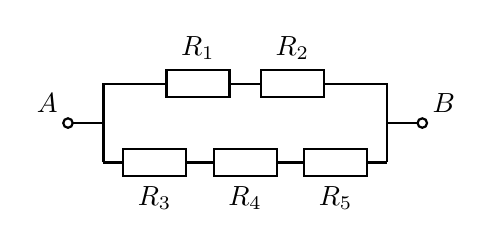
\begin{tikzpicture}[x=1cm,y=1cm,>=stealth,line width=0.8pt]
\draw (0,0) circle (0.06) node[above left] {\(A\)};
\draw (0.06,0)--(0.45,0);
\draw (0.45,-0.5)--(0.45,0.5)--(1.25,0.5);
\draw (1.25,0.33) rectangle (2.05,0.67);
\node[above] at (1.65,0.67) {\(R_1\)};
\draw (2.05,0.5)--(2.45,0.5);
\draw (2.45,0.33) rectangle (3.25,0.67);
\node[above] at (2.85,0.67) {\(R_2\)};
\draw (3.25,0.5)--(4.05,0.5)--(4.05,-0.5);
\draw (0.45,-0.5)--(0.7,-0.5);
\draw (0.7,-0.67) rectangle (1.5,-0.33);
\node[below] at (1.1,-0.67) {\(R_3\)};
\draw (1.5,-0.5)--(1.85,-0.5);
\draw (1.85,-0.67) rectangle (2.65,-0.33);
\node[below] at (2.25,-0.67) {\(R_4\)};
\draw (2.65,-0.5)--(3,-0.5);
\draw (3,-0.67) rectangle (3.8,-0.33);
\node[below] at (3.4,-0.67) {\(R_5\)};
\draw (3.8,-0.5)--(4.05,-0.5);
\draw (4.05,0)--(4.44,0);
\draw (4.5,0) circle (0.06) node[above right] {\(B\)};
\end{tikzpicture}
\end{center} (в $\text{В}$).
}{
\smallskip\noindent\textbf{Решение от GPT}\par
В верхней ветви два одинаковых последовательных резистора, поэтому
\[
U_{AB}=2U_2=24\ \text{В}.
\]
На нижней ветви такое же напряжение, которое делится поровну между тремя одинаковыми резисторами:
\[
U_3=\frac{U_{AB}}{3}=8\ \text{В}.
\]
Ответ: \(8\,\text{В}\).
}

% Source 8D32C8: https://ege.fipi.ru/bank/questions.php?search=1&proj=BA1F39653304A5B041B656915DC36B38&qid=8D32C8
\BankTask{8D32C8}{
Через участок цепи (см. рисунок) течёт постоянный ток $I=4\,\text{А}$. Какую силу тока покажет включённый в эту цепь идеальный амперметр, если сопротивление каждого резистора $r=1\,\text{Ом}$?
\begin{center}
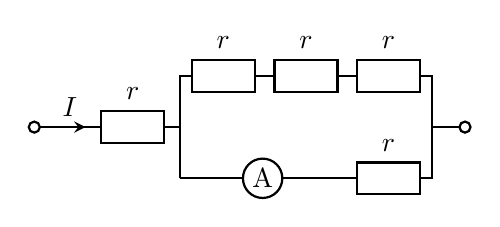
\begin{tikzpicture}[x=1cm,y=1cm,>=stealth,line width=0.8pt]
\draw (0,0) circle (0.07);
\draw (0.07,0)--(0.85,0);
\draw[->] (0.25,0)--(0.65,0) node[midway,above] {$I$};
\draw (0.85,-0.2) rectangle (1.65,0.2);
\node at (1.25,0.42) {$r$};
\draw (1.65,0)--(1.85,0);
\draw (1.85,-0.65)--(1.85,0.65)--(2,0.65);
\draw (2,0.45) rectangle (2.8,0.85);
\node at (2.4,1.07) {$r$};
\draw (2.8,0.65)--(3.05,0.65);
\draw (3.05,0.45) rectangle (3.85,0.85);
\node at (3.45,1.07) {$r$};
\draw (3.85,0.65)--(4.1,0.65);
\draw (4.1,0.45) rectangle (4.9,0.85);
\node at (4.5,1.07) {$r$};
\draw (4.9,0.65)--(5.05,0.65)--(5.05,-0.65)--(4.9,-0.65);
\draw (1.85,-0.65)--(2.65,-0.65);
\draw (2.9,-0.65) circle (0.25);
\node at (2.9,-0.65) {$\mathrm{A}$};
\draw (3.15,-0.65)--(4.1,-0.65);
\draw (4.1,-0.85) rectangle (4.9,-0.45);
\node at (4.5,-0.23) {$r$};
\draw (5.05,0)--(5.4,0);
\draw (5.47,0) circle (0.07);
\end{tikzpicture}
\end{center} (в $\text{А}$).
}{
\smallskip\noindent\textbf{Решение от GPT}\par
Сопротивления верхней и нижней параллельных ветвей равны $R_{\text{в}}=3r$ и $R_{\text{н}}=r$ (сопротивление идеального амперметра равно нулю). Поэтому $I_{\text{н}}/I_{\text{в}}=3$, а $I_{\text{н}}+I_{\text{в}}=I$. Показание амперметра:
\[
I_A=\frac{3}{4}I=3\,\text{А}.
\]
Ответ: $3\,\text{А}$.
}

% Source 45F97D: https://ege.fipi.ru/bank/questions.php?search=1&proj=BA1F39653304A5B041B656915DC36B38&qid=45F97D
\BankTask{45F97D}{
На фотографии изображена электрическая цепь. Показания вольтметра даны в вольтах, амперметра — в амперах.
\par\begin{center}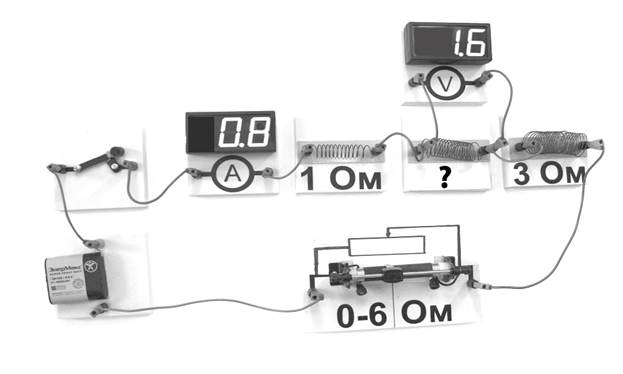
\includegraphics[width=.9\linewidth,height=.48\textheight,keepaspectratio]{_run/photos/11844cc09b6f9596afe3dd1ce24746ab1447feecb4b56a469c4f32a1860fabe4.png}\end{center}\par
Чему равно сопротивление неизвестного резистора (в $\text{Ом}$)? Вольтметр и амперметр считать идеальными.
}{
\smallskip\noindent\textbf{Решение от GPT}\par
По фотографии $I=0{,}8\,\text{А}$, $U=1{,}6\,\text{В}$. По закону Ома
\[
R=\frac{U}{I}=\frac{1{,}6}{0{,}8}=2\,\text{Ом}.
\]
}

% Source 9397C7: https://ege.fipi.ru/bank/questions.php?search=1&proj=BA1F39653304A5B041B656915DC36B38&qid=9397C7
\BankTask{9397C7}{
На фотографии изображена электрическая цепь. Показания вольтметра даны в вольтах.
\par\begin{center}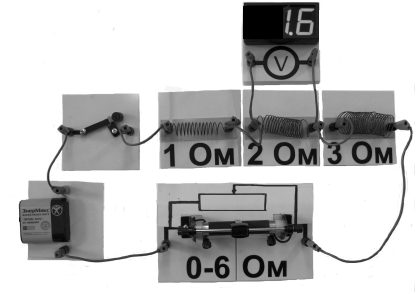
\includegraphics[width=.9\linewidth,height=.48\textheight,keepaspectratio]{_run/photos/389e5d4777aabc394c4661c2152661a8d428c2674ff93ab9ac03afcbdf49c8ea.png}\end{center}\par
Какое напряжение (в $\text{В}$) будет показывать вольтметр, если его подсоединить к резистору сопротивлением $3\,\text{Ом}$? Вольтметр считать идеальным.
}{
\smallskip\noindent\textbf{Решение от GPT}\par
На резисторе $2\,\text{Ом}$ вольтметр показывает $1{,}6\,\text{В}$. Ток в последовательно соединённых резисторах одинаков:
\[
I=\frac{1{,}6}{2}=0{,}8\,\text{А},\qquad U_3=I R_3=0{,}8\cdot3=2{,}4\,\text{В}.
\]
}

% Source D35A43: https://ege.fipi.ru/bank/questions.php?search=1&proj=BA1F39653304A5B041B656915DC36B38&qid=D35A43
\BankTask{D35A43}{
Восемь одинаковых резисторов с сопротивлением $r=1\,\text{Ом}$ соединены в электрическую цепь, через которую течёт ток $I=4\,\text{А}$ (см. рисунок). Какое напряжение (в $\text{В}$) показывает идеальный вольтметр?
\begin{center}
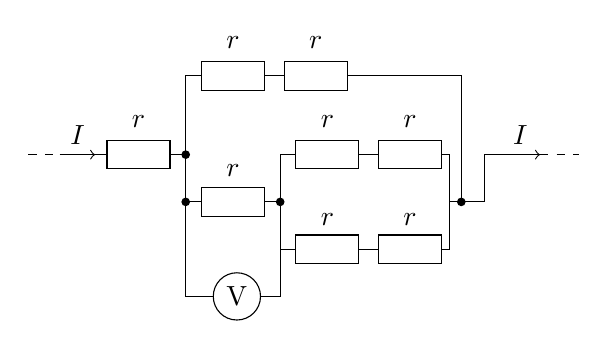
\begin{tikzpicture}[x=1cm,y=1cm]
\draw[dashed] (-1,0)--(-0.6,0);
\draw[->] (-0.6,0)--(-0.15,0) node[midway,above] {$I$};
\draw (-0.15,0)--(0,0);
\draw (0,-0.18) rectangle (0.8,0.18);
\node at (0.4,0.42) {$r$};
\draw (0.8,0)--(1,0)--(1,1)--(1.2,1);
\draw (1.2,0.82) rectangle (2,1.18);
\node at (1.6,1.42) {$r$};
\draw (2,1)--(2.25,1);
\draw (2.25,0.82) rectangle (3.05,1.18);
\node at (2.65,1.42) {$r$};
\draw (3.05,1)--(4.5,1)--(4.5,-0.6);
\draw (1,0)--(1,-0.6)--(1.2,-0.6);
\draw (1.2,-0.78) rectangle (2,-0.42);
\node at (1.6,-0.2) {$r$};
\draw (2,-0.6)--(2.2,-0.6);
\draw (2.2,-0.6)--(2.2,0)--(2.4,0);
\draw (2.4,-0.18) rectangle (3.2,0.18);
\node at (2.8,0.42) {$r$};
\draw (3.2,0)--(3.45,0);
\draw (3.45,-0.18) rectangle (4.25,0.18);
\node at (3.85,0.42) {$r$};
\draw (4.25,0)--(4.35,0)--(4.35,-0.6)--(4.5,-0.6);
\draw (2.2,-0.6)--(2.2,-1.2)--(2.4,-1.2);
\draw (2.4,-1.38) rectangle (3.2,-1.02);
\node at (2.8,-0.82) {$r$};
\draw (3.2,-1.2)--(3.45,-1.2);
\draw (3.45,-1.38) rectangle (4.25,-1.02);
\node at (3.85,-0.82) {$r$};
\draw (4.25,-1.2)--(4.35,-1.2)--(4.35,-0.6);
\draw (1,-0.6)--(1,-1.8)--(1.35,-1.8);
\draw (1.65,-1.8) circle (0.3);
\node at (1.65,-1.8) {$\mathrm{V}$};
\draw (1.95,-1.8)--(2.2,-1.8)--(2.2,-0.6);
\draw (4.5,-0.6)--(4.8,-0.6)--(4.8,0)--(5,0);
\draw[->] (5,0)--(5.5,0) node[midway,above] {$I$};
\draw[dashed] (5.5,0)--(6,0);
\foreach \x/\y in {1/0,1/-0.6,2.2/-0.6,4.5/-0.6} \fill (\x,\y) circle (0.055);
\end{tikzpicture}
\end{center}
}{
\smallskip\noindent\textbf{Решение от GPT}\par
Идеальный вольтметр тока не проводит. Две правые ветви имеют сопротивления $2r$ каждая, поэтому их параллельное соединение имеет сопротивление $r$. Нижняя ветвь между левым и правым узлами имеет сопротивление $r+r=2r$, верхняя — также $2r$. Ток делится поровну. Через резистор, к которому подключён вольтметр, течёт $I/2$:
\[
U=\frac{I}{2}r=\frac{4}{2}\cdot1=2\,\text{В}.
\]
}

\end{document}
